\section{Metodología de integración}

% Explica el proceso de construcción de la base de datos:
% - Cómo se alinearon las fuentes espacial y temporalmente
% - Procesos de limpieza, normalización o filtrado
% - Qué herramientas o lenguajes usaste (Python, QGIS, R, etc.)
% - Cómo se validó la integridad del conjunto de datos (valores faltantes, duplicados)
% - Cuál fue la lógica para estructurar los registros: por parcela, especie, clase diamétrica, etc.


La construcción de la base de datos se fundamenta en la integración de múltiples fuentes de información, alineadas espacial y temporalmente sobre una unidad básica común: la parcela del Inventario Forestal Nacional (IFN). Cada parcela está georreferenciada con coordenadas precisas, lo que permite su identificación única y la vinculación con otras capas de información espacial y temporal. Esta georreferenciación, junto con la fecha de muestreo (año de apeo), actúa como nexo de unión entre todos los conjuntos de datos empleados, posibilitando una articulación coherente y robusta de la información recopilada.

\medskip

Para cada una de las tres campañas del IFN consideradas (IFN2, IFN3 e IFN4), se toma el año de muestreo como referencia temporal. A partir de esta fecha se consulta, enlaza o calcula la información correspondiente de las demás fuentes. Así, por ejemplo, los datos meteorológicos y climáticos se extraen considerando el año anterior al muestreo, ya sea a nivel estacional o anual según la variable, mientras que las imágenes aéreas o satelitales se seleccionan para fechas cercanas al año de inventario. Esta estrategia garantiza que la información vinculada sea representativa del estado de la parcela en el momento del muestreo forestal.

\medskip

Desde el punto de vista técnico, el proceso de integración se llevó a cabo íntegramente en Python, apoyándose en bibliotecas como \texttt{pandas} y \texttt{geopandas} para la manipulación de datos tabulares y espaciales, \texttt{shapely} para el tratamiento geométrico, \texttt{owslib} y \texttt{PIL} para la descarga y procesamiento de imágenes aéreas, y \texttt{xarray} o \texttt{netCDF4} para la gestión de archivos climáticos multibanda. Adicionalmente, se emplearon herramientas SIG como QGIS de forma auxiliar para la validación visual de coberturas.

\medskip

La estructura de la base resultante se organiza jerárquicamente por parcela, inventario,  especie y clase diamétrica. Las tablas principales responden a claves compuestas que representan la identidad única de cada unidad de observación: \texttt{parcela}, \texttt{parcela\_inventario}, \texttt{parcela\_inventario\_especie} y \texttt{parcela\_inventario\_especie\_cd}. Además se incluye una tabla \texttt{parcela\_inventario\_estacion} en la que se almacenan los datos meteorológicos y satelitales de cada parcela que dependen de la estación. Durante el proceso de construcción se detectaron duplicidades en estas claves, causadas por errores de origen en los datos o repeticiones exactas. En una primera etapa se eliminaron todas las filas duplicadas completas. Posteriormente, para cada clave primaria compuesta, se retuvo únicamente el registro con menor número de valores ausentes (\texttt{NaN}), descartando los duplicados menos informativos.


\subsection{Preprocesado de los datos}

\subsubsection{Datos satelitales}

Todo el preprocesado de los datos satelitales se realiza con la herramienta \textit{Google Earth Engine}. A lo largo del preprocesamiento de los datos procedentes de satélites nos encontramos varios apartados. Para el caso de las imágenes:

\begin{itemize}
    \item \textbf{Eliminación de nubes y sombras, y enmascaramiento de los huecos}

    Con este paso tratamos de identificar y enmascarar píxeles que contienen nubes y sombras de nubes, los cuáles no nos dan información fiable sobre la superficie terrestre. Lo logramos seleccionando la banda de control de calidad QA\_PIXEL de la imagen, donde bits específicos indican la presencia de nubes (bit 5) y sombras de nubes (bit 3). Mediante operaciones lógicas bit a bit, cramos una máscara que marca como ``verdaderos'' (limpios) solo los píxeles libres de nubes y sombras. Finalmente, esta máscara se aplica a la imagen original, haciendo que las áreas afectadas por nubes y sombras se vuelvan transparentes o ``sin datos'', lo cual es esencial para asegurar análisis posteriores de la superficie terrestre sin interferencias atmosféricas. Un ejemplo de conjunto de datos para la primavera de $2004$ se puede ver en la Figura \ref{fig:imagenes_sat_primavera_2004}.

    \begin{figure}[H]
        \centering
        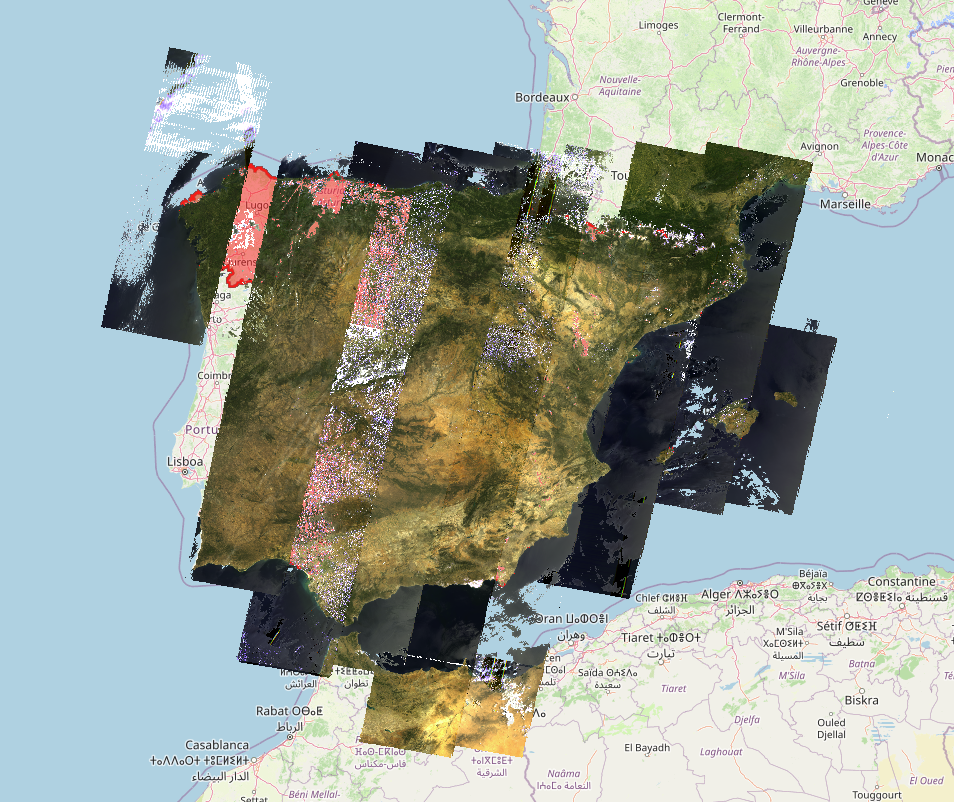
\includegraphics[width=0.7\linewidth]{figuras/ejemplo_imagen_sat_mala_calidad.png}
        \caption{Ejemplo de un conjunto de imágenes tras la eliminación de las nubes para la primavera de $2004$, que constituye un caso paradigmático del peor de los casos, en el que hay muchos huecos en las imágenes, para que se vea el procesado. Generalmente los datos son de mayor calidad (menos huecos) para el resto de años. Imágenes obtenidas del conjunto de datos Landsat 7 cortesía del Servicio Geológico de Estados Unidos.}
        \label{fig:imagenes_sat_primavera_2004}
    \end{figure}


    Si el periodo de observación que tomamos es relativamente corto (menos de 6 meses) y coincide con meses en los que suele haber más nubes, como es el otoño e invierno, nos encontraremos zonas en las que no tendremos observaciones, es decir, para una cierta zona no ha coincidido la pasada del satélite con un momento en el que no haya nubes. Para poder identificar estas zonas, identificaremos a estos puntos con el valor $-999$ para poder identificarlos claramente. También, para que esta situación se de lo menos posible, las imágenes de satélites las tomaremos solo para las estaciones de primavera y verano. 

    \item \textbf{Aplicación del factor de escala}

    La manera en la que están guardados los datos en el archivo original no representan directamente la reflectancia de la superficie o la temperatura en unidades físicas, principalmente por razones de eficiencia de almacenamiento, mantenimiento de precisión y similar. Para obtener valores con significado físico tenemos que aplicar una transformación lineal a los datos, la cuál podemos encontrar en la documentación del dataset, que es la siguiente:
    \begin{itemize}
        \item Transformación para las bandas ópticas (SR\_B):
        \[
        f(x) = 0.0000275x - 0.2.
        \]
        \item Transformación para las bandas térmicas (ST\_B6):
        \[
        f(x) = 0.00341802x + 149.
        \]
    \end{itemize}
    \item \textbf{Cálculo de los índices y otras medidas}\label{sec:indices}
    
    El siguiente paso es calcular los distintos índices vegetales que vamos a incorporar al modelo. Este proceso consiste en una serie de operaciones con algunas de las bandas del satélite según las longitudes de onda que éstas observen.

    \begin{itemize}
        \item \textbf{NDVI (Normalized Difference Vegetation Index)} \cite{eos_blog}
        
        El NDVI es uno de los más adecuados para seguir la dinámica de desarrollo de la vegetación, ya que mide la biomasa fotosintéticamente activa de las plantas. Sin embargo, este índice de vegetación es bastante sensible a la luminosidad del suelo y a los efectos atmosféricos, mitigados en otros índices como EVI.
        
        \[
        \text{NDVI} = \frac{\text{NIR} - \text{Red}}{\text{NIR} + \text{Red}} = \frac{\text{SR\_B4} - \text{SR\_B3}}{\text{SR\_B4} + \text{SR\_B3}}.
        \]
    
        \item \textbf{NDII (Normalized Index)} \cite{sentinel_hub_ndii}
        
        Es una medición de reflectancia, sensible a los cambios en el contenido de agua de los doseles vegetales. Los valores del índice aumentan con el incremento del contenido de agua. Las aplicaciones del NDII incluyen la gestión de cultivos agrícolas, el monitoreo de las copas de los árboles y la detección de vegetación estresada.
        \[
        \text{NDII} = \frac{\text{NIR} - \text{SWIR}}{\text{NIR} + \text{SWIR}} = \frac{\text{SR\_B4} - \text{SR\_B5}}{\text{SR\_B4} + \text{SR\_B5}}.
        \]
    
        \item \textbf{GNDVI (Green Normalized Difference Vegetation Index) } \cite{eos_indices_vegetacion}
        
        El índice GNDVI es una modificación del NDVI que también utiliza el infrarrojo cercano, pero sustituye el verde visible por el rojo visible. Suele emplearse para detectar cultivos marchitos o envejecidos y medir el contenido de nitrógeno en las hojas cuando no se dispone de un canal rojo extremo, monitorizar la vegetación con copas densas o en las etapas de madurez.
        \[
        \text{GNDVI} = \frac{\text{NIR} - \text{GREEN}}{\text{NIR} + \text{GREEN}} = \frac{\text{SR\_B4} - \text{SR\_B2}}{\text{SR\_B4} + \text{SR\_B2}}.
        \]
    
        \item \textbf{EVI (Enhanced Vegetation Index)} \cite{eos_indices_vegetacion}
        
        Se creó para ajustar los resultados del NDVI a los ruidos atmosféricos y del suelo, especialmente en las zonas de vegetación densa, así como para mitigar la saturación en la mayoría de los casos.
        
        \begin{align}
             \text{EVI} &= 2.5 \left( \frac{\text{NIR} - \text{RED}}{\text{NIR} + C_1 \cdot \text{RED} - C_2 \cdot \text{BLUE} + L} \right ), \\
             & = 2.5 \left( \frac{\text{SR\_B4 - SR\_B3}}{\text{SR\_B4} + C_1 \cdot \text{SR\_B3} - C_2 \cdot \text{SR\_B1 + L}} \right),
        \end{align}
   
        donde \(C_1 = 6\), \(C_2 = 7.5\) y \(L = 1\). El índice EVI contiene los coeficientes \(C_1\) y \(C_2\) para corregir la dispersión de los aerosoles presentes en la atmósfera y \(L\) para ajustar el fondo del suelo y las copas de la vegetación.
    
        \item \textbf{SLOPE (Pendiente)} \cite{ee_terrain_slope}
        
        Partiendo de un Mapa Digital de Terreno (DEM, por sus siglas en inglés) el gradiente local se calcula utilizando los 4 vecinos conectados de cada píxel, por lo que se producirán valores faltantes alrededor de los bordes de una imagen. El cálculo se realiza mediante la función \texttt{ee.Terrain.slope} de \textit{Google Earth Engine}.
    
        \item \textbf{ASPECT (Orientación)} \cite{ee_terrain_slope}
        
        De igual forma que para el caso anterior, este dato se calcula a partir de Mapa Digital de Terreno calculando el gradiente utilizando los 4 vecinos conectados de cada píxel. Se empleó la función \texttt{ee.Terrain.aspect} de \textit{Google Earth Engine}.
    \end{itemize}

Una vez realizado este proceso solo quedaría extraer el valor para las latitudes y longitudes que deseemos. 


\subsubsection{Inventario Forestal Nacional}

El objetivo de los siguientes pasos es la criba de los datos, eliminación e imputación de faltantes y la generación de identificadores únicos para las entradas de cada tabla. Tras este preprocesamiento se obtienen cuatro tablas con sus correspondientes identificadores únicos y con datos cribados. Se normalizan los códigos de las especies, se completan datos como las etiquetas de carbono y se estima la superficie de cada parcela.


\begin{itemize}
    \item \textbf{Creación de identificadores para cada tabla.} Para facilitar el manejo de los datos lo primero que se hace es crear un identificador para cada parcela. Esto se lleva a cabo concatenando \texttt{Estadillo} y \texttt{Provincia}. Este identificador debe tratarse con mucha atención pues es lo que permitirá relacionar las observaciones de uno y otro inventario. A partir de esta clave se construyen las claves primarias de cada tabla que deben ser tratadas para asegurar su unicidad: \texttt{idparcela\_inventario}, \texttt{idparcela\_inventario\_especie} e \texttt{idparcela\_inventario\_especie\_cd}.
    
    \medskip
    
    \item \textbf{Normalización de los códigos de las especies.} Se normaliza la codificación de las especies para que coincidan entre inventarios siguiendo la Tabla \ref{tab:codificacion_especies}. 

    
    \medskip

    \item \textbf{Filtrado por las coordenadas de las parcelas. } Eliminamos las parcelas que no tengan unas coordenadas válidas ($\texttt{CoorX}, \texttt{CoorY} =0$ o faltante). Consideramos dos parcelas como coincidentes entre dos inventarios cuando  tienen un mismo \texttt{idparcela} y sus coordenadas (tanto en X como en Y) estan a una distancia inferior a $300$m. Eliminamos las parcelas que no estén en al menos dos inventarios. Las coordenadas de los inventarios son progresivamente más precisas, siendo las coordenadas del cuarto inventario las mejores. Como, una vez filtradas, se considera una única ubicación para cada parcela, empleamos las coordenadas del inventario cuarto por defecto. En caso de no existir se emplean las coordenadas del inventario tercero, nunca las del segundo. 

    \medskip
    
    \item \textbf{Corrección en el huso geográfico.} Al proyectar las coordenadas de las parcelas sobre el mapa encontramos muchos errores (parcelas sobre el mar, en otros países o sobre la provincia equivocada). Tras la exploración de los datos encontramos que los errores se deben a una mala asignación de los husos geográficos. Vemos en la figura \ref{fig:husos} estas divisiones del territorio. 
    \begin{figure}[H]
        \centering
        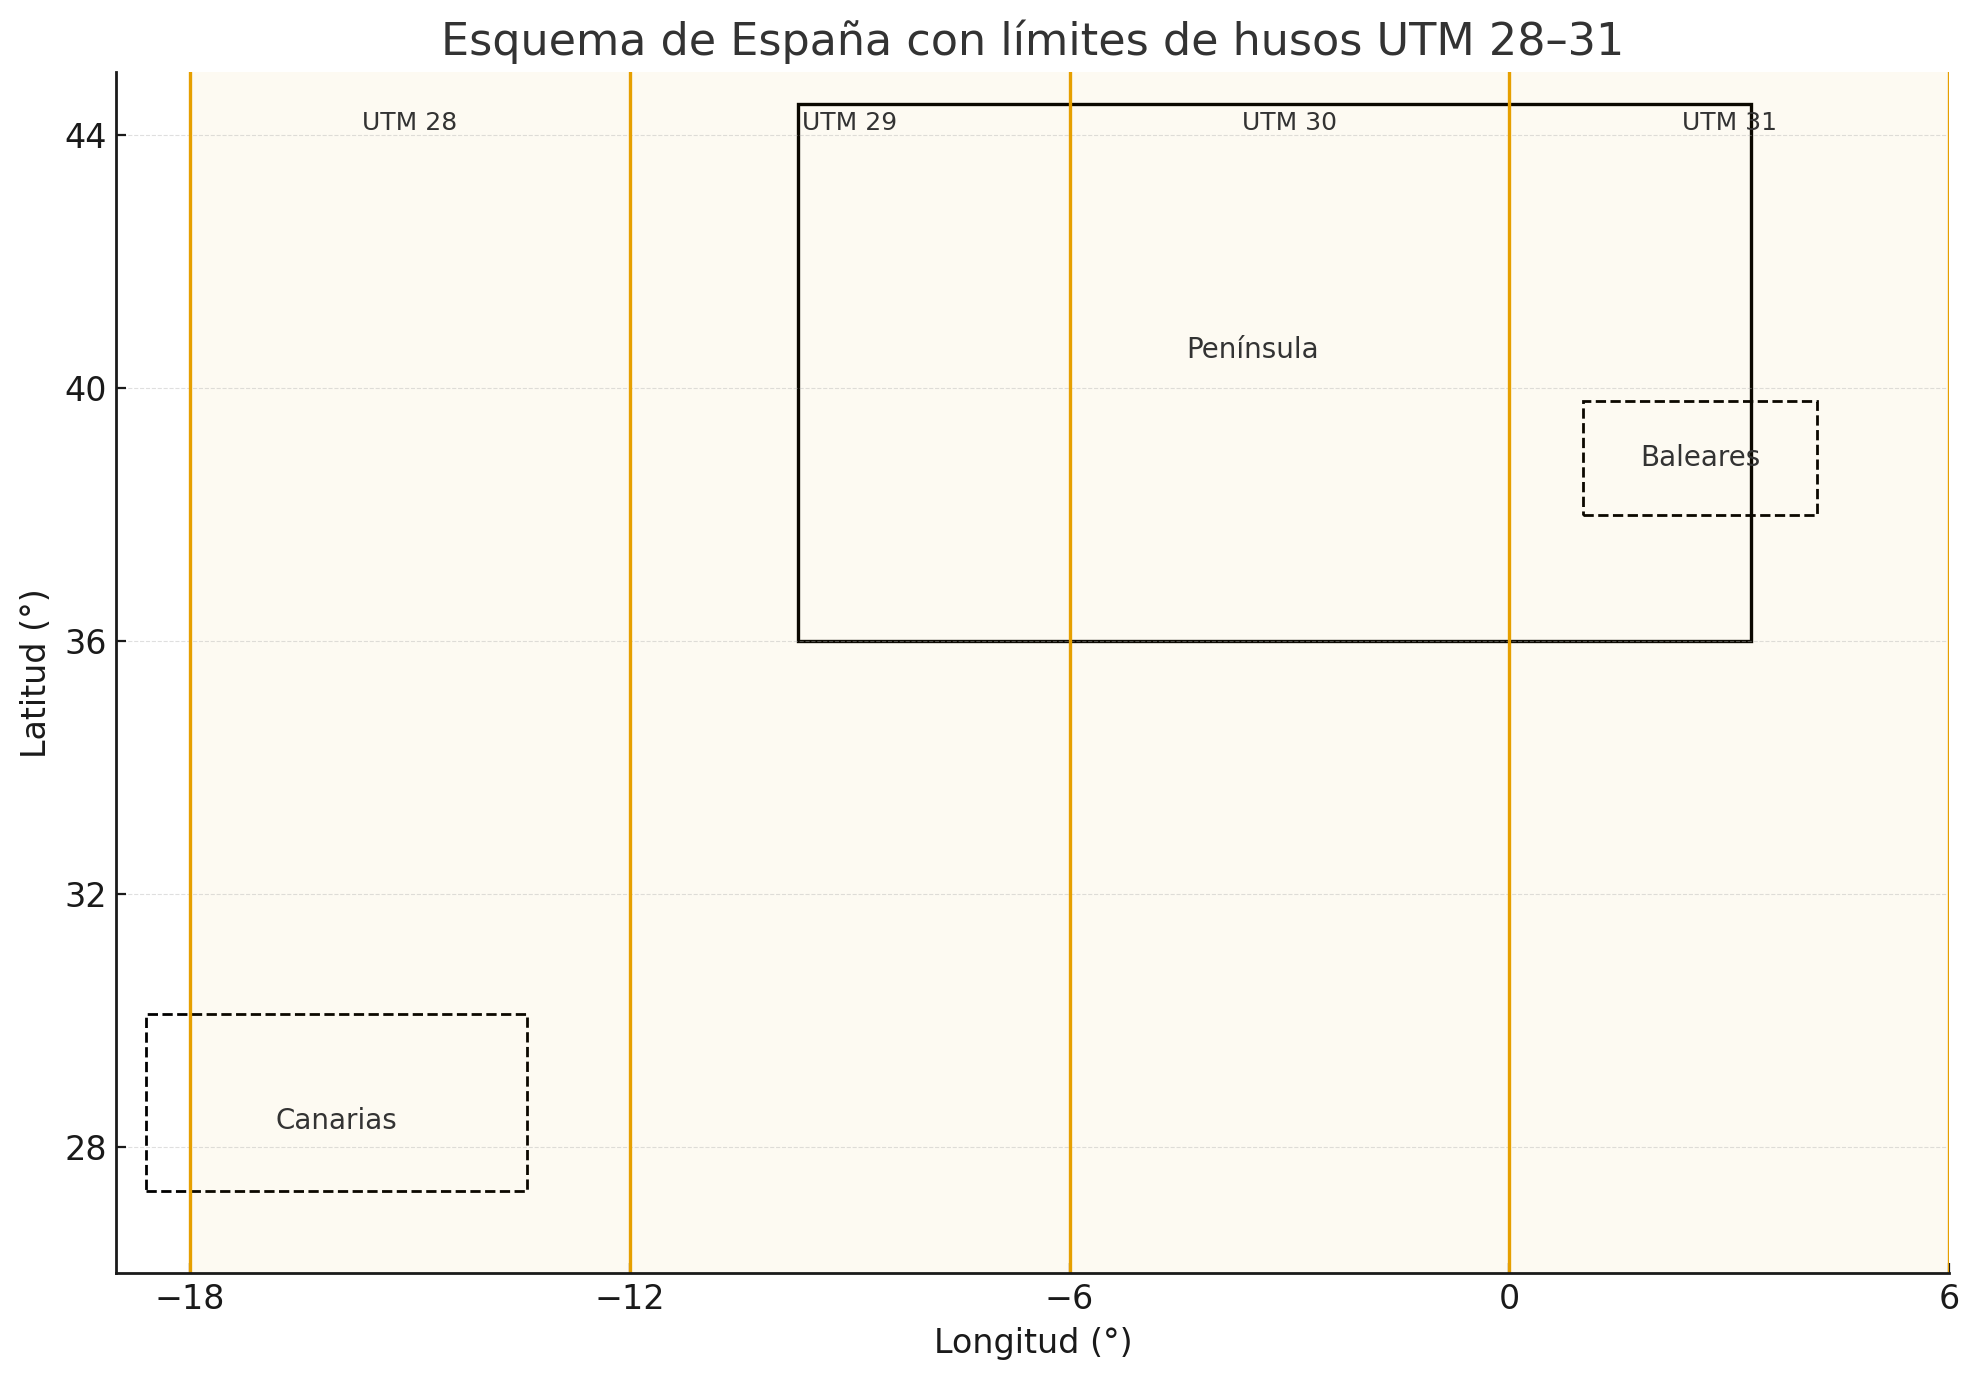
\includegraphics[width=0.4\textwidth]{figuras/husos.jpeg}
        \caption{\small Imagen del mapa peninsular con los husos geográficos. Se contemplan las bandas de huso 29, 30 y 31. Las islas Canarias no aparecen en la imagen pero sí que se contemplan en la base de datos (huso 28 y 29).}
        \label{fig:husos}
    \end{figure}
    
    Algunas de las provincias atravesadas por una de estas limitaciones geográficas mantienen el mismo valor de \texttt{Huso} para todas sus parcelas, no adaptandose al cambio en la proyección. Para identificar las parcelas mal proyectadas empleamos el \textbf{shapefile de la Base de Datos de Divisiones Administrativas de España} \cite{ign_shapefile}, de donde podemos obtener un rango en longitud y altitud de cada provincia. Corregimos el huso de aquellas parcelas cuya longitud esta fuera del rango de longitud de su provincia (la corrección es sencilla porque sabiendo cual es la provincia sabemos que frontera de huso la atraviesa). Eliminamos las parcelas que, una vez corregidas, tienen una longitud o latitud fuera de los rangos del territorio español. 

    \medskip

    \item \textbf{Filtrado por año de exploración.} Se eliminan los registros de las parcelas (entradas de las tablas cuya clave primaria contiene el inventario) anteriores a 1950. No existen datos de satélite para estos años y se sospecha que la mayoría de estas observaciones son erróneas. 

    \medskip
    
    \item \textbf{Incorporación de pies menores a \texttt{parcela\_inventario\_especie\_cd}.} Los datos de la tabla \texttt{brotes} (\ref{tab:brotes}) permiten identificar y caracterizar los cultivos forestales en su fase inicial. Esta tabla, como se puede consultar en el anexo \ref{sec:CatDesDensidad}, incluye un recuento de los especímenes de entre $30$ cm y $1,3$ m o aquellos de altura superior pero diámetro del tronco inferior a $7,5$ cm. Sin embargo, el recuento de pies por clase diamétrica incluido en la tabla \texttt{parcela\_inventario\_especie\_cd} (Tabla \ref{tab:parcela_inventario_especie_cd}) parten de una clase diamétrica igual a $10$ cm. Los datos de la tabla \texttt{brotes} se incorporan a la tabla \texttt{parcela\_inventario\_especie\_cd} (tabla \ref{tab:parcela_inventario_especie_cd}) de la siguiente manera: 
    
    \medskip
    
    Cada entrada de la tabla \texttt{brotes} corresponde a un conjunto de árboles de una parcela, inventario y especie concreta y se caracteriza por la variable \texttt{CatDes} o categoría del desarrollo: 
    
    \begin{enumerate}
        \item Pies con altura inferior a $30$ cm.
        \item Pies con altura comprendida entre $30$ y $130$ cm.
        \item Pies con altura superior a 130 cm y diámetro normal menor de $2,5$ cm.
        \item Pies con altura superior a $130$ cm y diámetro normal comprendido entre $2,5$ y $7,5$ cm. Corresponde a los pies menores del IFN2.
    \end{enumerate}
    
    \medskip
    
    Para añadir dichas entradas a la tabla \texttt{parcela\_inventario\_especie\_cd} (Tabla \ref{tab:parcela_inventario_especie_cd}) es necesario definir una clase diamétrica y estimar un número de pies para cada entrada/grupo de árboles. Mapeamos la variable \texttt{CatDes} a la clase diamétrica: Los valores de categoría del desarrollo $1$ y $2$ se asignan como \texttt{CD}$=1$, los valores $3$ se asignan como \texttt{CD}$=2$ y los valores $4$ se asignan como \texttt{CD}$=5$. 
    
    \medskip
    
    El número de árboles de cada grupo se extrae de la variable \texttt{Densidad}, esta se cuantifica según la categoría de desarrollo:
    
    \medskip
    
    \textbf{Para las categorías $1, 2$ y $3$}:
    \begin{enumerate}
        \item \textbf{Escasa:} De $1$ a $4$ pies en la parcela.
        \item \textbf{Normal:} De $5$ a $15$ pies en la parcela.
        \item \textbf{Abundante:} Más de $15$ pies en la parcela.
    
    \medskip
    
    \end{enumerate}
    \textbf{Para la categoría 4:}
    \begin{itemize}
        \item Se cuenta el número exacto de pies por especie en la subparcela de 5 m de radio. Se registra en la casilla ``NPies''.
    \end{itemize}
    
    \medskip
    
    Así, se ajusta el número de árboles de cada grupo según el valor de \texttt{Densidad}. Si el valor de \texttt{Densidad} es 1, 2 o 3, se asignan valores específicos a \texttt{NPies} (2.5, 10 y 15, respectivamente); de lo contrario, se conserva el valor original de \texttt{NumPies}.
    
    \medskip

    \item \textbf{Variables \texttt{CA} y \texttt{CR}.} Estas variables (carbono arbolado y carbono radical por hectárea\footnote{Diferenciamos entre la fijación de carbono aéreo del arbolado y la fijación de carbono radical del arbolado, dos componentes distintos del almacenamiento total de carbono en un ecosistema forestal. La fijación de carbono aéreo se refiere a la cantidad de carbono almacenado en la biomasa aérea del arbolado (tronco, ramas, hojas) y la fijación de carbono radical a la cantidad de carbono almacenado en el sistema radical (raíces); representan el 70-80\% y el 20-30\% del carbono total del árbol respectivamente. Ambos son relevantes, pero el carbono aéreo es el más comúnmente contabilizado en proyectos de créditos de carbono por ser más fácil de contabilizar y de asegurar su permanencia. }) están registradas solo para el IFN4 para cada grupo de árboles de una clase diamétrica y especie concreta (tabla \texttt{parcela\_especie\_inventario\_cd} (\ref{tab:parcela_inventario_especie_cd}) restringida al inventario cuarto) y se calculan usando la Guía para la estimación de absorciones de dióxido de carbono propuesta por el MITECO \cite{miteco_guia_co2}. 

    \medskip

    Algunas provincias (las provincias $07, 15, 27, 30, 31, 32, 33, 36, 39$ y del País Vasco) no tienen las variables \texttt{CA} y \texttt{CR} registradas por lo que es necesario estimarlas. Para solucionar estos faltantes, además de los debidos a fallos en la recogida de los datos, se emplea un  modelo \textit{RandomForestRegressor}
\footnote{Para evaluar el modelo se dividen los datos en un $80\%$ para entrenamiento y un $20\%$ para validación. El modelo para \texttt{CA} obtiene: $\text{MSE}_{\text{CA, train}}= 0.28$, $\text{MSE}_{\text{CA, test}} = 5.48$, $R^2_{\text{CA, train}} = 0.99$, $R^2_{\text{CA, test}} = 0.91$. Para \texttt{CR}, las métricas son: $\text{MSE}_{\text{CR, train}}= 0.24$, $\text{MSE}_{\text{CR, test}}= 1.34$, $R^2_{\text{CR, train}} = 0.99$, $R^2_{\text{CR, test}} = 0.94$.}
, que permite predecir estos valores a partir de las características disponibles en los datos. El modelo se entrena utilizando un conjunto de variables predictoras, que incluyen \texttt{Especie,  CD, VSC, NPies, ABas, IAVC, VCC} y \texttt{VLE}. Este mismo modelo se aplica para asignar etiquetas de carbono a los datos del inventario tercero y segundo (IFN2 e IFN3). Los datos provenientes de la tabla \texttt{brotes} (Tabla \ref{tab:brotes}) se consideran de carbono $0$. 

\medskip

\item \textbf{Creación de la variable \texttt{c} (carbono).} Creamos la variable \texttt{c} que será la variable objetivo del modelo como \texttt{c=CA+CR} para cada entrada de la tabla \texttt{parcela\_inventario\_especie\_cd} (tabla \ref{tab:parcela_inventario_especie_cd}). Los valores de estas variables se registran en toneladas por hectárea y, por tanto, para generalizar a las entradas de la tabla \texttt{parcela\_inventario\_especie} (Tabla \ref{tab:parcela_inventario_especie}) solo se requiere agrupar en \texttt{parcela\_inventario\_especie\_cd} por especie y sumar los valores de \texttt{c}.

\item \textbf{Filtrado por valores de \texttt{c} y número de árboles.} Se eliminan de la base de datos las parcelas que no registran carbono capturado en ningún inventario (\texttt{c} igual a 0 en IFN2, IFN3 e IFN4). Además, se eliminan las especies de las parcelas que no tienen registro en ninguno de los inventarios de la presencia de árboles (aquellos valores de \texttt{parcela\_inventario\_especie} no presentes en \texttt{parcela\_inventario\_especie\_cd}). 

\medskip

\item \textbf{Estimación de la superficie de la parcela.} El IFN no proporciona las dimensiones de cada parcela registrada. Para estimar este dato empleamos la variable \texttt{Distanci} de la tabla parcela (\ref{tab:parcela}). Las coordenadas de cada parcela registran el punto central de la parcela y de la documentación de los inventarios se entiende que se trata de parcelas circulares. La variable \texttt{Distanci} registra un conjunto de medidas correspondientes a la distancia entre cada pie mayor contenido en la parcela y el centro de la misma. Estimamos el radio de la parcela como la mayor de dichas distancias (distancia entre el centro de la parcela y el árbol más alejado contenido en ella). Registramos las variables \texttt{Radio} en metros y la variable \texttt{Superficie} en hectáreas. Las parcelas que no cuentan con mediciones de \texttt{Distanci} validas se imputan con la media. 
 
\end{itemize}
